\documentclass[12pt]{article}

%packages
%\usepackage{latexsym}
\usepackage{graphicx}
\usepackage{color}
\usepackage{amsmath}
%\usepackage{dsfont}
\usepackage{placeins}
\usepackage{amssymb}
\usepackage{wasysym}
\usepackage{abstract}
\usepackage{hyperref}

%\usepackage{pstricks,pst-node,pst-tree}

%\usepackage{algpseudocode}
%\usepackage{amsthm}
%\usepackage{hyperref}
%\usepackage{mathrsfs}
%\usepackage{amsfonts}
%\usepackage{bbding}
%\usepackage{listings}
%\usepackage{appendix}
\usepackage[margin=1in]{geometry}
%\geometry{papersize={8.5in,11in},total={6.5in,9in}}
%\usepackage{cancel}
%\usepackage{algorithmic, algorithm}

\newcounter{probnum}
\setcounter{probnum}{1}

%create definition to allow local margin changes
\def\changemargin#1#2{\list{}{\rightmargin#2\leftmargin#1}\item[]}
\let\endchangemargin=\endlist 

%allow equations to span multiple pages
\allowdisplaybreaks

%define colors and color typesetting conveniences
\definecolor{gray}{rgb}{0.5,0.5,0.5}
\definecolor{black}{rgb}{0,0,0}
\definecolor{white}{rgb}{1,1,1}
\definecolor{blue}{rgb}{0.5,0.5,1}
\newcommand{\inblue}[1]{\color{blue}#1 \color{black}}
\definecolor{green}{rgb}{0.133,0.545,0.133}
\newcommand{\ingreen}[1]{\color{green}#1 \color{black}}
\definecolor{yellow}{rgb}{1,0.549,0}
\newcommand{\inyellow}[1]{\color{yellow}#1 \color{black}}
\definecolor{red}{rgb}{1,0.133,0.133}
\newcommand{\inred}[1]{\color{red}#1 \color{black}}
\definecolor{purple}{rgb}{0.58,0,0.827}
\newcommand{\inpurple}[1]{\color{purple}#1 \color{black}}
\definecolor{backgcode}{rgb}{0.97,0.97,0.8}
\definecolor{Brown}{cmyk}{0,0.81,1,0.60}
\definecolor{OliveGreen}{cmyk}{0.64,0,0.95,0.40}
\definecolor{CadetBlue}{cmyk}{0.62,0.57,0.23,0}

%define new math operators
\DeclareMathOperator*{\argmax}{arg\,max~}
\DeclareMathOperator*{\argmin}{arg\,min~}
\DeclareMathOperator*{\argsup}{arg\,sup~}
\DeclareMathOperator*{\arginf}{arg\,inf~}
\DeclareMathOperator*{\convolution}{\text{\Huge{$\ast$}}}
\newcommand{\infconv}[2]{\convolution^\infty_{#1 = 1} #2}
%true functions

%%%% GENERAL SHORTCUTS

%shortcuts for pure typesetting conveniences
\newcommand{\bv}[1]{\boldsymbol{#1}}

%shortcuts for compound constants
\newcommand{\BetaDistrConst}{\dfrac{\Gamma(\alpha + \beta)}{\Gamma(\alpha)\Gamma(\beta)}}
\newcommand{\NormDistrConst}{\dfrac{1}{\sqrt{2\pi\sigma^2}}}

%shortcuts for conventional symbols
\newcommand{\tsq}{\tau^2}
\newcommand{\tsqh}{\hat{\tau}^2}
\newcommand{\sigsq}{\sigma^2}
\newcommand{\sigsqsq}{\parens{\sigma^2}^2}
\newcommand{\sigsqovern}{\dfrac{\sigsq}{n}}
\newcommand{\tausq}{\tau^2}
\newcommand{\tausqalpha}{\tau^2_\alpha}
\newcommand{\tausqbeta}{\tau^2_\beta}
\newcommand{\tausqsigma}{\tau^2_\sigma}
\newcommand{\betasq}{\beta^2}
\newcommand{\sigsqvec}{\bv{\sigma}^2}
\newcommand{\sigsqhat}{\hat{\sigma}^2}
\newcommand{\sigsqhatmlebayes}{\sigsqhat_{\text{Bayes, MLE}}}
\newcommand{\sigsqhatmle}[1]{\sigsqhat_{#1, \text{MLE}}}
\newcommand{\bSigma}{\bv{\Sigma}}
\newcommand{\bSigmainv}{\bSigma^{-1}}
\newcommand{\thetavec}{\bv{\theta}}
\newcommand{\thetahat}{\hat{\theta}}
\newcommand{\thetahatmle}{\hat{\theta}_{\mathrm{MLE}}}
\newcommand{\thetavechatmle}{\hat{\thetavec}_{\mathrm{MLE}}}
\newcommand{\muhat}{\hat{\mu}}
\newcommand{\musq}{\mu^2}
\newcommand{\muvec}{\bv{\mu}}
\newcommand{\muhatmle}{\muhat_{\text{MLE}}}
\newcommand{\lambdahat}{\hat{\lambda}}
\newcommand{\lambdahatmle}{\lambdahat_{\text{MLE}}}
\newcommand{\etavec}{\bv{\eta}}
\newcommand{\alphavec}{\bv{\alpha}}
\newcommand{\minimaxdec}{\delta^*_{\mathrm{mm}}}
\newcommand{\ybar}{\bar{y}}
\newcommand{\xbar}{\bar{x}}
\newcommand{\Xbar}{\bar{X}}
\newcommand{\iid}{~{\buildrel iid \over \sim}~}
\newcommand{\inddist}{~{\buildrel ind \over \sim}~}
\newcommand{\approxdist}{~{\buildrel approx \over \sim}~}
\newcommand{\equalsindist}{~{\buildrel d \over =}~}
\newcommand{\loglik}[1]{\ell\parens{#1}}
\newcommand{\thetahatkminone}{\thetahat^{(k-1)}}
\newcommand{\thetahatkplusone}{\thetahat^{(k+1)}}
\newcommand{\thetahatk}{\thetahat^{(k)}}
\newcommand{\half}{\frac{1}{2}}
\newcommand{\third}{\frac{1}{3}}
\newcommand{\twothirds}{\frac{2}{3}}
\newcommand{\fourth}{\frac{1}{4}}
\newcommand{\fifth}{\frac{1}{5}}
\newcommand{\sixth}{\frac{1}{6}}

%shortcuts for vector and matrix notation
\newcommand{\A}{\bv{A}}
\newcommand{\At}{\A^T}
\newcommand{\Ainv}{\inverse{\A}}
\newcommand{\B}{\bv{B}}
\newcommand{\K}{\bv{K}}
\newcommand{\Kt}{\K^T}
\newcommand{\Kinv}{\inverse{K}}
\newcommand{\Kinvt}{(\Kinv)^T}
\newcommand{\M}{\bv{M}}
\newcommand{\Bt}{\B^T}
\newcommand{\Q}{\bv{Q}}
\newcommand{\Qt}{\Q^T}
\newcommand{\R}{\bv{R}}
\newcommand{\Rt}{\R^T}
\newcommand{\Z}{\bv{Z}}
\newcommand{\X}{\bv{X}}
\newcommand{\Xsub}{\X_{\text{(sub)}}}
\newcommand{\Xsubadj}{\X_{\text{(sub,adj)}}}
\newcommand{\I}{\bv{I}}
\newcommand{\Y}{\bv{Y}}
\newcommand{\sigsqI}{\sigsq\I}
\renewcommand{\P}{\bv{P}}
\newcommand{\Psub}{\P_{\text{(sub)}}}
\newcommand{\Pt}{\P^T}
\newcommand{\Pii}{P_{ii}}
\newcommand{\Pij}{P_{ij}}
\newcommand{\IminP}{(\I-\P)}
\newcommand{\Xt}{\bv{X}^T}
\newcommand{\XtX}{\Xt\X}
\newcommand{\XtXinv}{\parens{\Xt\X}^{-1}}
\newcommand{\XtXinvXt}{\XtXinv\Xt}
\newcommand{\XXtXinvXt}{\X\XtXinvXt}
\newcommand{\x}{\bv{x}}
\newcommand{\onevec}{\bv{1}}
\newcommand{\oneton}{1, \ldots, n}
\newcommand{\yoneton}{y_1, \ldots, y_n}
\newcommand{\yonetonorder}{y_{(1)}, \ldots, y_{(n)}}
\newcommand{\Yoneton}{Y_1, \ldots, Y_n}
\newcommand{\iinoneton}{i \in \braces{\oneton}}
\newcommand{\onetom}{1, \ldots, m}
\newcommand{\jinonetom}{j \in \braces{\onetom}}
\newcommand{\xoneton}{x_1, \ldots, x_n}
\newcommand{\Xoneton}{X_1, \ldots, X_n}
\newcommand{\xt}{\x^T}
\newcommand{\y}{\bv{y}}
\newcommand{\yt}{\y^T}
\renewcommand{\c}{\bv{c}}
\newcommand{\ct}{\c^T}
\newcommand{\tstar}{\bv{t}^*}
\renewcommand{\u}{\bv{u}}
\renewcommand{\v}{\bv{v}}
\renewcommand{\a}{\bv{a}}
\newcommand{\s}{\bv{s}}
\newcommand{\yadj}{\y_{\text{(adj)}}}
\newcommand{\xjadj}{\x_{j\text{(adj)}}}
\newcommand{\xjadjM}{\x_{j \perp M}}
\newcommand{\yhat}{\hat{\y}}
\newcommand{\yhatsub}{\yhat_{\text{(sub)}}}
\newcommand{\yhatstar}{\yhat^*}
\newcommand{\yhatstarnew}{\yhatstar_{\text{new}}}
\newcommand{\z}{\bv{z}}
\newcommand{\zt}{\z^T}
\newcommand{\bb}{\bv{b}}
\newcommand{\bbt}{\bb^T}
\newcommand{\bbeta}{\bv{\beta}}
\newcommand{\beps}{\bv{\epsilon}}
\newcommand{\bepst}{\beps^T}
\newcommand{\e}{\bv{e}}
\newcommand{\Mofy}{\M(\y)}
\newcommand{\KofAlpha}{K(\alpha)}
\newcommand{\ellset}{\mathcal{L}}
\newcommand{\oneminalph}{1-\alpha}
\newcommand{\SSE}{\text{SSE}}
\newcommand{\SSEsub}{\text{SSE}_{\text{(sub)}}}
\newcommand{\MSE}{\text{MSE}}
\newcommand{\RMSE}{\text{RMSE}}
\newcommand{\SSR}{\text{SSR}}
\newcommand{\SST}{\text{SST}}
\newcommand{\JSest}{\delta_{\text{JS}}(\x)}
\newcommand{\Bayesest}{\delta_{\text{Bayes}}(\x)}
\newcommand{\EmpBayesest}{\delta_{\text{EmpBayes}}(\x)}
\newcommand{\BLUPest}{\delta_{\text{BLUP}}}
\newcommand{\MLEest}[1]{\hat{#1}_{\text{MLE}}}

%shortcuts for Linear Algebra stuff (i.e. vectors and matrices)
\newcommand{\twovec}[2]{\bracks{\begin{array}{c} #1 \\ #2 \end{array}}}
\newcommand{\threevec}[3]{\bracks{\begin{array}{c} #1 \\ #2 \\ #3 \end{array}}}
\newcommand{\fivevec}[5]{\bracks{\begin{array}{c} #1 \\ #2 \\ #3 \\ #4 \\ #5 \end{array}}}
\newcommand{\twobytwomat}[4]{\bracks{\begin{array}{cc} #1 & #2 \\ #3 & #4 \end{array}}}
\newcommand{\threebytwomat}[6]{\bracks{\begin{array}{cc} #1 & #2 \\ #3 & #4 \\ #5 & #6 \end{array}}}

%shortcuts for conventional compound symbols
\newcommand{\thetainthetas}{\theta \in \Theta}
\newcommand{\reals}{\mathbb{R}}
\newcommand{\complexes}{\mathbb{C}}
\newcommand{\rationals}{\mathbb{Q}}
\newcommand{\integers}{\mathbb{Z}}
\newcommand{\naturals}{\mathbb{N}}
\newcommand{\forallninN}{~~\forall n \in \naturals}
\newcommand{\forallxinN}[1]{~~\forall #1 \in \reals}
\newcommand{\matrixdims}[2]{\in \reals^{\,#1 \times #2}}
\newcommand{\inRn}[1]{\in \reals^{\,#1}}
\newcommand{\mathimplies}{\quad\Rightarrow\quad}
\newcommand{\mathlogicequiv}{\quad\Leftrightarrow\quad}
\newcommand{\eqncomment}[1]{\quad \text{(#1)}}
\newcommand{\limitn}{\lim_{n \rightarrow \infty}}
\newcommand{\limitN}{\lim_{N \rightarrow \infty}}
\newcommand{\limitd}{\lim_{d \rightarrow \infty}}
\newcommand{\limitt}{\lim_{t \rightarrow \infty}}
\newcommand{\limitsupn}{\limsup_{n \rightarrow \infty}~}
\newcommand{\limitinfn}{\liminf_{n \rightarrow \infty}~}
\newcommand{\limitk}{\lim_{k \rightarrow \infty}}
\newcommand{\limsupn}{\limsup_{n \rightarrow \infty}}
\newcommand{\limsupk}{\limsup_{k \rightarrow \infty}}
\newcommand{\floor}[1]{\left\lfloor #1 \right\rfloor}
\newcommand{\ceil}[1]{\left\lceil #1 \right\rceil}

%shortcuts for environments
\newcommand{\beqn}{\vspace{-0.25cm}\begin{eqnarray*}}
\newcommand{\eeqn}{\end{eqnarray*}}
\newcommand{\bneqn}{\vspace{-0.25cm}\begin{eqnarray}}
\newcommand{\eneqn}{\end{eqnarray}}

%shortcuts for mini environments
\newcommand{\parens}[1]{\left(#1\right)}
\newcommand{\squared}[1]{\parens{#1}^2}
\newcommand{\tothepow}[2]{\parens{#1}^{#2}}
\newcommand{\prob}[1]{\mathbb{P}\parens{#1}}
\newcommand{\littleo}[1]{o\parens{#1}}
\newcommand{\bigo}[1]{O\parens{#1}}
\newcommand{\Lp}[1]{\mathbb{L}^{#1}}
\renewcommand{\arcsin}[1]{\text{arcsin}\parens{#1}}
\newcommand{\prodonen}[2]{\bracks{\prod_{#1=1}^n #2}}
\newcommand{\mysum}[4]{\sum_{#1=#2}^{#3} #4}
\newcommand{\sumonen}[2]{\sum_{#1=1}^n #2}
\newcommand{\infsum}[2]{\sum_{#1=1}^\infty #2}
\newcommand{\infprod}[2]{\prod_{#1=1}^\infty #2}
\newcommand{\infunion}[2]{\bigcup_{#1=1}^\infty #2}
\newcommand{\infinter}[2]{\bigcap_{#1=1}^\infty #2}
\newcommand{\infintegral}[2]{\int^\infty_{-\infty} #2 ~\text{d}#1}
\newcommand{\supthetas}[1]{\sup_{\thetainthetas}\braces{#1}}
\newcommand{\bracks}[1]{\left[#1\right]}
\newcommand{\braces}[1]{\left\{#1\right\}}
\newcommand{\set}[1]{\left\{#1\right\}}
\newcommand{\abss}[1]{\left|#1\right|}
\newcommand{\norm}[1]{\left|\left|#1\right|\right|}
\newcommand{\normsq}[1]{\norm{#1}^2}
\newcommand{\inverse}[1]{\parens{#1}^{-1}}
\newcommand{\rowof}[2]{\parens{#1}_{#2\cdot}}

%shortcuts for functionals
\newcommand{\realcomp}[1]{\text{Re}\bracks{#1}}
\newcommand{\imagcomp}[1]{\text{Im}\bracks{#1}}
\newcommand{\range}[1]{\text{range}\bracks{#1}}
\newcommand{\colsp}[1]{\text{colsp}\bracks{#1}}
\newcommand{\rowsp}[1]{\text{rowsp}\bracks{#1}}
\newcommand{\tr}[1]{\text{tr}\bracks{#1}}
\newcommand{\rank}[1]{\text{rank}\bracks{#1}}
\newcommand{\proj}[2]{\text{Proj}_{#1}\bracks{#2}}
\newcommand{\projcolspX}[1]{\text{Proj}_{\colsp{\X}}\bracks{#1}}
\newcommand{\median}[1]{\text{median}\bracks{#1}}
\newcommand{\mean}[1]{\text{mean}\bracks{#1}}
\newcommand{\dime}[1]{\text{dim}\bracks{#1}}
\renewcommand{\det}[1]{\text{det}\bracks{#1}}
\newcommand{\expe}[1]{\mathbb{E}\bracks{#1}}
\newcommand{\expeabs}[1]{\expe{\abss{#1}}}
\newcommand{\expesub}[2]{\mathbb{E}_{#1}\bracks{#2}}
\newcommand{\indic}[1]{\mathds{1}_{#1}}
\newcommand{\var}[1]{\mathbb{V}\text{ar}\bracks{#1}}
\newcommand{\sd}[1]{\mathbb{S}\text{D}\bracks{#1}}
\newcommand{\cov}[2]{\text{Cov}\bracks{#1, #2}}
\newcommand{\corr}[2]{\text{Corr}\bracks{#1, #2}}
\newcommand{\se}[1]{\text{SE}\bracks{#1}}
\newcommand{\seest}[1]{\hat{\text{SE}}\bracks{#1}}
\newcommand{\bias}[1]{\text{Bias}\bracks{#1}}
\newcommand{\partialop}[2]{\dfrac{\partial}{\partial #1}\bracks{#2}}
\newcommand{\secpartialop}[2]{\dfrac{\partial^2}{\partial #1^2}\bracks{#2}}
\newcommand{\mixpartialop}[3]{\dfrac{\partial^2}{\partial #1 \partial #2}\bracks{#3}}

%shortcuts for functions
\renewcommand{\exp}[1]{\mathrm{exp}\parens{#1}}
\renewcommand{\cos}[1]{\text{cos}\parens{#1}}
\renewcommand{\sin}[1]{\text{sin}\parens{#1}}
\newcommand{\sign}[1]{\text{sign}\parens{#1}}
\newcommand{\are}[1]{\mathrm{ARE}\parens{#1}}
\newcommand{\natlog}[1]{\ln\parens{#1}}
\newcommand{\oneover}[1]{\frac{1}{#1}}
\newcommand{\overtwo}[1]{\frac{#1}{2}}
\newcommand{\overn}[1]{\frac{#1}{n}}
\newcommand{\oneoversqrt}[1]{\oneover{\sqrt{#1}}}
\newcommand{\sqd}[1]{\parens{#1}^2}
\newcommand{\loss}[1]{\ell\parens{\theta, #1}}
\newcommand{\losstwo}[2]{\ell\parens{#1, #2}}
\newcommand{\cf}{\phi(t)}

%English language specific shortcuts
\newcommand{\ie}{\textit{i.e.} }
\newcommand{\AKA}{\textit{AKA} }
\renewcommand{\iff}{\textit{iff}}
\newcommand{\eg}{\textit{e.g.} }
\newcommand{\st}{\textit{s.t.} }
\newcommand{\wrt}{\textit{w.r.t.} }
\newcommand{\mathst}{~~\text{\st}~~}
\newcommand{\mathand}{~~\text{and}~~}
\newcommand{\ala}{\textit{a la} }
\newcommand{\ppp}{posterior predictive p-value}
\newcommand{\dd}{dataset-to-dataset}

%shortcuts for distribution titles
\newcommand{\logistic}[2]{\mathrm{Logistic}\parens{#1,\,#2}}
\newcommand{\bernoulli}[1]{\mathrm{Bernoulli}\parens{#1}}
\newcommand{\betanot}[2]{\mathrm{Beta}\parens{#1,\,#2}}
\newcommand{\stdbetanot}{\betanot{\alpha}{\beta}}
\newcommand{\multnormnot}[3]{\mathcal{N}_{#1}\parens{#2,\,#3}}
\newcommand{\normnot}[2]{\mathcal{N}\parens{#1,\,#2}}
\newcommand{\classicnormnot}{\normnot{\mu}{\sigsq}}
\newcommand{\stdnormnot}{\normnot{0}{1}}
\newcommand{\uniform}[2]{\mathrm{U}\parens{#1,\,#2}}
\newcommand{\stduniform}{\uniform{0}{1}}
\newcommand{\exponential}[1]{\mathrm{Exp}\parens{#1}}
\newcommand{\gammadist}[2]{\mathrm{Gamma}\parens{#1, #2}}
\newcommand{\poisson}[1]{\mathrm{Poisson}\parens{#1}}
\newcommand{\binomial}[2]{\mathrm{Binomial}\parens{#1,\,#2}}
\newcommand{\rayleigh}[1]{\mathrm{Rayleigh}\parens{#1}}
\newcommand{\multinomial}[2]{\mathrm{Multinomial}\parens{#1,\,#2}}
\newcommand{\gammanot}[2]{\mathrm{Gamma}\parens{#1,\,#2}}
\newcommand{\cauchynot}[2]{\text{Cauchy}\parens{#1,\,#2}}
\newcommand{\invchisqnot}[1]{\text{Inv}\chisq{#1}}
\newcommand{\invscaledchisqnot}[2]{\text{ScaledInv}\ncchisq{#1}{#2}}
\newcommand{\invgammanot}[2]{\text{InvGamma}\parens{#1,\,#2}}
\newcommand{\chisq}[1]{\chi^2_{#1}}
\newcommand{\ncchisq}[2]{\chi^2_{#1}\parens{#2}}
\newcommand{\ncF}[3]{F_{#1,#2}\parens{#3}}

%shortcuts for PDF's of common distributions
\newcommand{\logisticpdf}[3]{\oneover{#3}\dfrac{\exp{-\dfrac{#1 - #2}{#3}}}{\parens{1+\exp{-\dfrac{#1 - #2}{#3}}}^2}}
\newcommand{\betapdf}[3]{\dfrac{\Gamma(#2 + #3)}{\Gamma(#2)\Gamma(#3)}#1^{#2-1} (1-#1)^{#3-1}}
\newcommand{\normpdf}[3]{\frac{1}{\sqrt{2\pi#3}}\exp{-\frac{1}{2#3}(#1 - #2)^2}}
\newcommand{\normpdfvarone}[2]{\dfrac{1}{\sqrt{2\pi}}e^{-\half(#1 - #2)^2}}
\newcommand{\chisqpdf}[2]{\dfrac{1}{2^{#2/2}\Gamma(#2/2)}\; {#1}^{#2/2-1} e^{-#1/2}}
\newcommand{\invchisqpdf}[2]{\dfrac{2^{-\overtwo{#1}}}{\Gamma(#2/2)}\,{#1}^{-\overtwo{#2}-1}  e^{-\oneover{2 #1}}}
\newcommand{\exponentialpdf}[2]{#2\exp{-#2#1}}
\newcommand{\poissonpdf}[2]{\dfrac{e^{-#1} #1^{#2}}{#2!}}
\newcommand{\binomialpdf}[3]{\binom{#2}{#1}#3^{#1}(1-#3)^{#2-#1}}
\newcommand{\rayleighpdf}[2]{\dfrac{#1}{#2^2}\exp{-\dfrac{#1^2}{2 #2^2}}}
\newcommand{\gammapdf}[3]{\dfrac{#3^#2}{\Gamma\parens{#2}}#1^{#2-1}\exp{-#3 #1}}
\newcommand{\cauchypdf}[3]{\oneover{\pi} \dfrac{#3}{\parens{#1-#2}^2 + #3^2}}
\newcommand{\Gammaf}[1]{\Gamma\parens{#1}}

%shortcuts for miscellaneous typesetting conveniences
\newcommand{\notesref}[1]{\marginpar{\color{gray}\tt #1\color{black}}}

%%%% DOMAIN-SPECIFIC SHORTCUTS

%Real analysis related shortcuts
\newcommand{\zeroonecl}{\bracks{0,1}}
\newcommand{\forallepsgrzero}{\forall \epsilon > 0~~}
\newcommand{\lessthaneps}{< \epsilon}
\newcommand{\fraccomp}[1]{\text{frac}\bracks{#1}}

%Bayesian related shortcuts
\newcommand{\yrep}{y^{\text{rep}}}
\newcommand{\yrepisq}{(\yrep_i)^2}
\newcommand{\yrepvec}{\bv{y}^{\text{rep}}}


%Probability shortcuts
\newcommand{\SigField}{\mathcal{F}}
\newcommand{\ProbMap}{\mathcal{P}}
\newcommand{\probtrinity}{\parens{\Omega, \SigField, \ProbMap}}
\newcommand{\convp}{~{\buildrel p \over \rightarrow}~}
\newcommand{\convLp}[1]{~{\buildrel \Lp{#1} \over \rightarrow}~}
\newcommand{\nconvp}{~{\buildrel p \over \nrightarrow}~}
\newcommand{\convae}{~{\buildrel a.e. \over \longrightarrow}~}
\newcommand{\convau}{~{\buildrel a.u. \over \longrightarrow}~}
\newcommand{\nconvau}{~{\buildrel a.u. \over \nrightarrow}~}
\newcommand{\nconvae}{~{\buildrel a.e. \over \nrightarrow}~}
\newcommand{\convd}{~{\buildrel \mathcal{D} \over \rightarrow}~}
\newcommand{\nconvd}{~{\buildrel \mathcal{D} \over \nrightarrow}~}
\newcommand{\withprob}{~~\text{w.p.}~~}
\newcommand{\io}{~~\text{i.o.}}

\newcommand{\Acl}{\bar{A}}
\newcommand{\ENcl}{\bar{E}_N}
\newcommand{\diam}[1]{\text{diam}\parens{#1}}

\newcommand{\taua}{\tau_a}

\newcommand{\myint}[4]{\int_{#2}^{#3} #4 \,\text{d}#1}
\newcommand{\laplacet}[1]{\mathscr{L}\bracks{#1}}
\newcommand{\laplaceinvt}[1]{\mathscr{L}^{-1}\bracks{#1}}
\renewcommand{\min}[1]{\text{min}\braces{#1}}

\newcommand{\Vbar}[1]{\bar{V}\parens{#1}}
\newcommand{\expnegrtau}{\exp{-r\tau}}

%%% problem typesetting
\newcommand{\problem}{\vspace{0.2cm} \noindent {\large{\textsf{Problem \arabic{probnum}~}}} \addtocounter{probnum}{1}}
%\newcommand{\easyproblem}{\ingreen{\noindent \textsf{Problem \arabic{probnum}~}} \addtocounter{probnum}{1}}
%\newcommand{\intermediateproblem}{\noindent \inyellow{\textsf{Problem \arabic{probnum}~}} \addtocounter{probnum}{1}}
%\newcommand{\hardproblem}{\inred{\noindent \textsf{Problem \arabic{probnum}~}} \addtocounter{probnum}{1}}
%\newcommand{\extracreditproblem}{\noindent \inpurple{\textsf{Problem \arabic{probnum}~}} \addtocounter{probnum}{1}}

\newcommand{\easysubproblem}{\ingreen{\item}}
\newcommand{\intermediatesubproblem}{\inyellow{\item}}
\newcommand{\hardsubproblem}{\inred{\item}}
\newcommand{\extracreditsubproblem}{\inpurple{\item}}
\renewcommand{\labelenumi}{(\alph{enumi})}


\title{Statistics 101 Summer I 2011 \\ Homework \#2}
\author{Adam Kapelner, Instructor}

\date{Due 1PM, Thursday, June 9, 2011 (in my mail slot)}

\renewcommand{\abstractname}{Instructions and Philosophy}

\begin{document}
\maketitle


\begin{abstract}
It's easy for me to pretend to teach and you to pretend to learn. It's hard for me to actually teach and for you to actually learn. This requires you to put in a lot of work. This homework is very long but it will really teach you the material. I strongly suggest you start early and \textit{work in teams}; do not do this one solo.

In Stine \& Foster, read sections 9.1--9.4, 10.1, 10.3, 10.5 (ignore everything about joint distributions, covariances, and dependent random variables), then 11.1--11.4, then loop back and read ch. 1--4 and stop at p.63 (do not read about the empirical rule). Section 4.2 is about histograms, so please read that carefully.

Once again, \ingreen{green} means \textit{easy}, \inyellow{yellow} means \textit{intermediate}, \inred{red} means \textit{difficult}, and \inpurple{purple} means \textit{extra credit}. This homework is worth 100 points but the point distribution will not be determined until after the due date. Late homework will be penalized 10 points per day. Beyond Friday June 10 at 5PM, it will receive a zero. 15 points are given as a bonus if the homework is typed using \LaTeX ~(please comment out all extraneous text).
\end{abstract}

\paragraph{Fundamentals of Random Variables} Problems below are related to the fundamentals of r.v.'s which you'll find mostly in ch. 9 of S\&F. This section will also cover rules of expectation, variance, and summing r.v.'s found in ch. 10. \\

\problem Imagine rolling two dice. Let $X_1$ be the r.v. corresponding to the first die and let $X_2$ be the r.v. corresponding to the second die. Let the outcomes be \$1 if you roll a 1, \$2 if you roll a 2, \ldots, and \$6 if you roll a six.

\begin{figure}[htp]
\centering
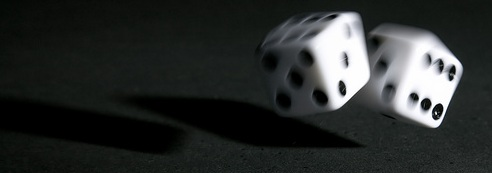
\includegraphics[width=3in, height=1.035in]{dice.jpg}
\end{figure}
\FloatBarrier

\begin{enumerate}
\easysubproblem Are these two r.v.'s independent? Identically distributed? Are $X_1, X_2 \iid$?

\easysubproblem Find $\expe{X_1}$, $\var{X_1}$, $\sd{X_1}$.
\easysubproblem Draw the probability mass function (PMF) to scale of $X_1$ similar to how we did in class (see p.199). 
\easysubproblem Draw the PMF of $2X_1$.
\easysubproblem Imagine a new r.v., call it $Y$, where you make \$11 if you roll a 1, \$14 if roll a 2, \ldots, and \$26 if you roll a 6. Express $Y$ as a function of $X_1$. Using elementary transformation theory, find $\expe{Y}$, $\var{Y}$, $\sd{Y}$.
\intermediatesubproblem Define a new r.v. $S = X_1 + X_2$. Using the methods in class, find its PMF and then draw it to scale.
\easysubproblem What is the support of $S$?
\easysubproblem Calculate $\expe{S}$ from first principles and $\var{S}, \sd{S}$ from the formulas.
\end{enumerate}

\problem We will investigate some basic facts of mathematical statistics. Consider $\Xoneton \iid$(some PMF) with nonzero mean $\mu$ and nonzero variance $\sigsq$.


\begin{enumerate}
\easysubproblem Define $S_n$ as we did in class. and compute $\expe{S_n}$, $\var{S_n}$, $\sd{S_n}$. 
\easysubproblem Calculate all three of the following:

\beqn
\limitn \expe{S_n}, \quad \limitn \var{S_n}, \quad \limitn \sd{S_n}
\eeqn

Why do your answers make sense?

\easysubproblem Define $\Xbar_n$ as we did in class and compute $\expe{\Xbar_n}$, $\var{\Xbar_n}$, $\sd{\Xbar_n}$. 
\easysubproblem Calculate all three of the following:

\beqn
\limitn \expe{\Xbar_n}, \quad \limitn \var{\Xbar_n}, \quad \limitn \sd{\Xbar_n}
\eeqn

Why do your answers make sense?

%\intermediatesubproblem Draw the limiting density of $\expe{\Xbar_n}$ (\ie the PMF in the limit of $n$ going to infinity). Label your axes clearly; label the support clearly.
%
%\intermediatesubproblem Repeat part (e) for $\sd{\Xbar_n}$. Does your picture make sense? Why?

\hardsubproblem Prove from the definition of variance that $\var{X} = \expe{X^2} - \mu^2$. This is a very useful formula that you should add to your toolbox.

\extracreditsubproblem Let $X, Y$ be discrete r.v.'s just like we are used to in class. Prove $\expe{X+Y} = \expe{X} + \expe{Y}$ from first principles. Super-hard... but if you slog through it, you will have a good command of density functions.
\extracreditsubproblem Why does $s^2$ have the correction factor of $\oneover{n-1}$? Read up on \href{http://en.wikipedia.org/wiki/Bessel's\_correction}{Bessel's correction}. Define what a ``biased estimator'' is and prove that $s^2$ is unbiased. Do not attempt this unless you are \textit{already done} with the assignment.
\end{enumerate}
\pagebreak
\problem We are going to learn the casino game of Roulette.

\begin{figure}[htp]
\centering
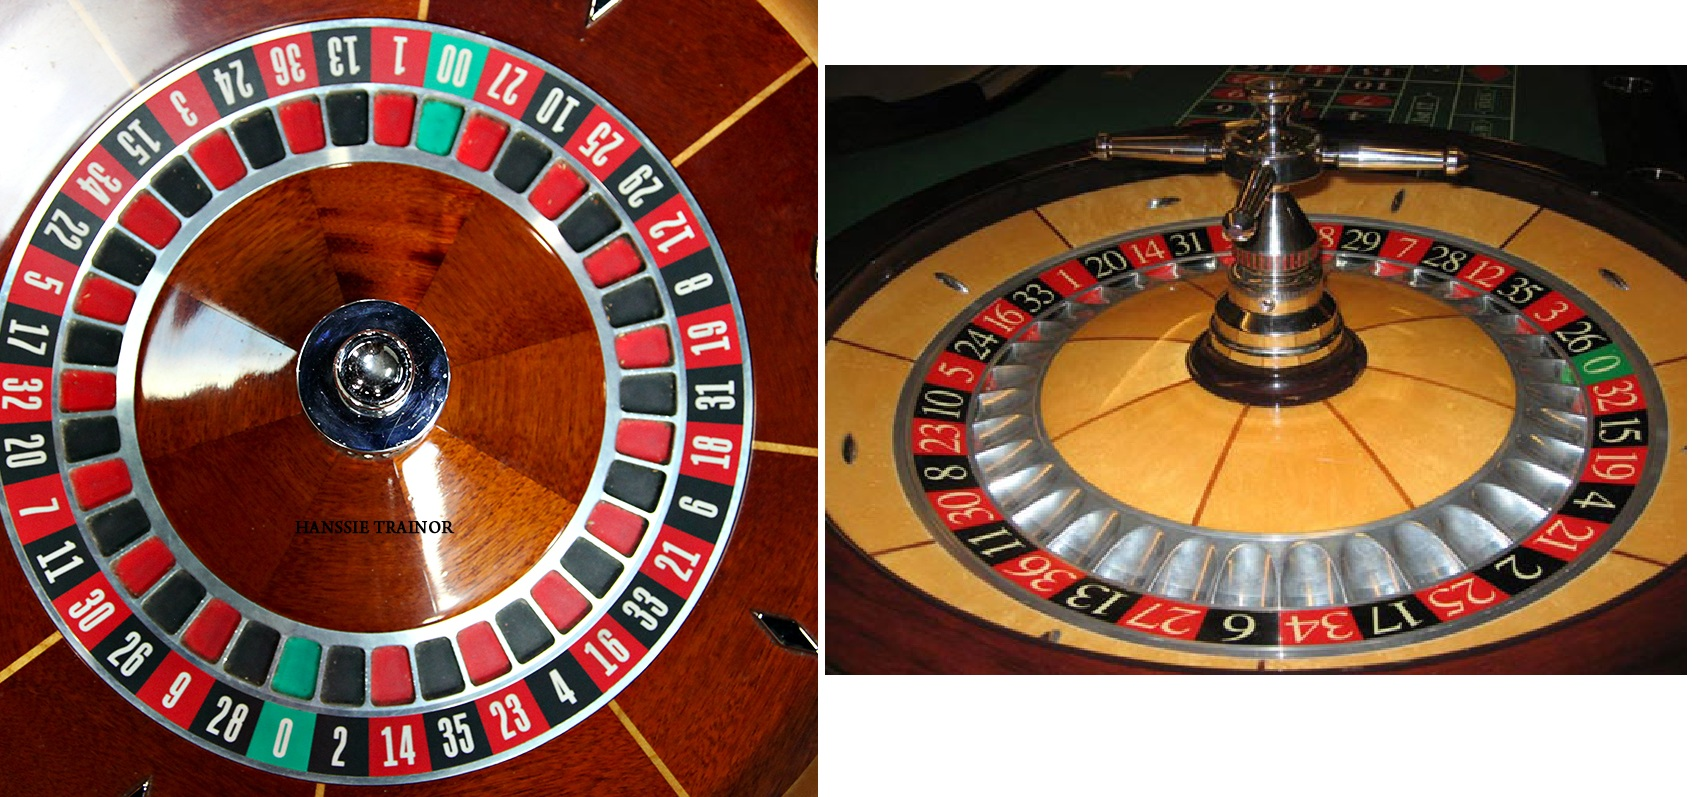
\includegraphics[width=4in, height=1.88in]{roulette.jpg}
\end{figure}
\FloatBarrier

\noindent The figure on the left is an American Roulette wheel; the figure on the right is a European Roulette wheel. American Roulette has 38 pockets and European Roulette has 37 pockets. Consider the standard bet of \$5.
\begin{enumerate}
\easysubproblem Create a r.v. $X$ for betting on the ball landing in black on an American Roulette table. The payoff is 1:1. Use the $\sim$ and piecewise function notation from class. Think carefully about what losing is: how much do you lose? How much do you win? This will enable you to get the outcomes / states of $X$.
\easysubproblem Draw the PMF and calculate $\expe{X}$, $\var{X}$, $\sd{X}$ from first principles. Indicate $\mu$ on the PMF with the fulcrum symbol like we did in class.
\easysubproblem Now, model $Y$, one bet of \$10,000 on black and an entrance of \$10 to the casino. Calculate $\expe{Y}$ and $\var{Y}$ using elementary transformation theory.
\intermediatesubproblem Now, model $V$, one bet of \$10,000 on black with a tip to the cashier of \$200 \textit{if} you win. Calculate $\expe{V}$.
\easysubproblem Repeat part (b) for a European Roulette wheel. 
\easysubproblem Would you rather play Roulette in America or Europe? Why?
\hardsubproblem What is the expected \textit{average} of 100 bets on the number 17? The payoff there is 35:1 and the bet is still \$5 and we are playing in Las Vegas.
\end{enumerate}

\begin{figure}[htp]
\centering
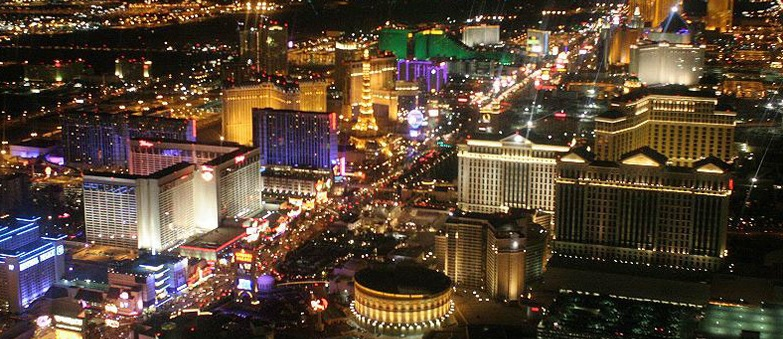
\includegraphics[width=4in, height=1.73in]{vegas.jpg}
\end{figure}
\FloatBarrier


%%%last
\problem In the finance industry, Sharpe ratios are traditionally used to compare mutual funds. In this problem we are going to compare funds \href{http://www.google.com/finance?q=JARTX}{JARTX} and \href{http://www.google.com/finance?q=VFAIX}{VFAIX} (click the links to search them on Google Finance). Both of these funds invest in large-cap US equities.

%wall street line
 
\begin{enumerate}
\easysubproblem Open \texttt{two\_mutual\_funds.JMP} which tabulates the date and the \textit{weekly} return rates for these two mutual funds. Multiply by 100 to get percentages. Now let JMP compute $\xbar$ and $s$ for both mutual funds using the ``analyze...distribution'' function. Calculate the Sharpe ratios for both mutual funds by using the formula from p.208 of F\&S. Use $\xbar$ to estimate $\expe{X}$ and $s$ to estimate $\sigma$. Use $r_{\text{f}}=0.0769\%$ as the ``risk free'' weekly interest rate.\footnote{This was calculated using 3-month T-bills, but that's not important for the scope of this class. In your finance classes you will cover this in more depth.}
\intermediatesubproblem If you had a choice between these two funds, which would you buy and why?
\end{enumerate}

\paragraph{Bernoullis, Binomials, and Poissons} In this section we will be covering the material in Chapter 11. \\

\problem Derivation of basic facts

\begin{enumerate}
\easysubproblem Let $S_n = X_1 + \ldots + X_n$ where $\Xoneton \iid \bernoulli{p}$. How is $S_n$ distributed? Indicate the parameter values clearly and explain them in your own words.
\intermediatesubproblem Rederive the PMF of the $\binomial{n}{p}$ just like we did in class from the notes. Explain each step. When you get the final PMF, label what each part of this function means in your own words.

\extracreditsubproblem Let $Y \sim \poisson{\lambda}$. Prove $\expe{Y} = \lambda$ from first principles \ie from the definition of expectation. This one is super hard. Do not do this unless you have hours to spare and wish to sharpen your algebra skills. This would be considered an intermediate problem in Stat 430 --- the course on probability. Hint: use the Taylor series: $e^x = \mysum{k}{0}{\infty}{\frac{x^k}{k!}}$ 

\end{enumerate}

\problem We will be investigating the situation where there are $n=1500$ students and $p=2\%$, the probability they enroll in Stat 101 in the summer. Assume each student is ruggedly individualistic about their choice of classes and they each have the same interest level in Statistics.

\begin{enumerate}
\easysubproblem Calculate the probability of 30 students enrolling in Stat 101. This is the expected number of students to enroll. Does the probability you calculated feel low to you? Explain.
\easysubproblem This is a case where $n$ is high and $p$ is low. Let $U$ be the r.v. that models the approximation we learned about in class. How is $U$ distributed? Indicate your parameters clearly.
\easysubproblem The \texttt{R} code below will graph the PMF of $Y \sim \binomial{1500}{2\%}$ in \inred{red} and the PMF of $U$ in \ingreen{green.} Copy and paste the code into the console. If this doesn't work, no excuses, copy and paste it to a text editor, format it exactly as you see below and try again.

\begin{verbatim}
n = 1500; 
p = 0.02; 
support_max = 300; 
bin = array(NA, support_max); 
pois = array(NA, support_max); 
for (i in 1 : support_max){
  bin[i] = dbinom(i, n, p); 
  pois[i] = dpois(i, n * p); 
}
plot(bin[1:60],
  pch = 16, 
  col = "red", 
  xlab = "Number of students enrolled in Stat 101", 
  ylab = "probability", 
  main = "Class Enrollment Probabilities for Stat 101"); 
points(pois[1:60], col = "green", pch = 16);
#placeholder for last line
\end{verbatim}

Is $U$ a good approximation of $Y$? Why or why not? Print out the plot and attach it to your homework.
\end{enumerate}


\begin{figure}[htp]
\centering
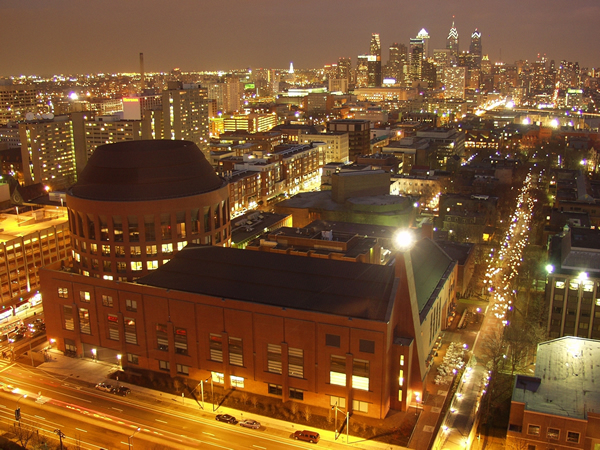
\includegraphics[width=2in, height=1.5in]{huntsman.jpg}
\end{figure}
\FloatBarrier

\paragraph{Data} We will be reviewing the concepts of data as realizations of r.v.'s and do some modeling in this section. \\

\problem On p197-198, F\&S investigate \href{http://finance.yahoo.com/q/hp?s=IBM+Historical+Prices}{IBM} stock returns by using a mock model. We're going to build a more believable statistical model by using real data for the past 100 trading days between Jan 7, 2011 and June 1, 2011. This will \textit{still} be a mock model. Building more believable models is what hedge fund dudes get paid the big bucks for.

\begin{figure}[htp]
\centering
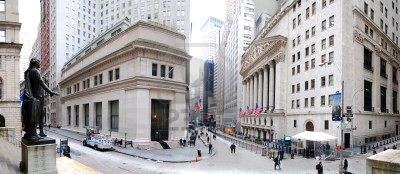
\includegraphics[width=3in, height=1.3in]{wallstreet.jpg}
\end{figure}
\FloatBarrier

\begin{enumerate}
\easysubproblem Go to the Yahoo Finance page  then click on ``historical prices'' on the left (you can click on the link above to go straight there). Query for the data between Jan 7, 2011 and June 1, 2011. Click the ``Download to Spreadsheet'' link. You now have the file \texttt{table.csv}. Open this up in JMP and sort so that the date Jan 7, 2011 is first. Now create a new column that calculates the daily returns \textit{as a percentage}. Use the \textit{adjusted closing} price\footnote{you will learn why this is different from the regular closing price in your finance class}. Now create a histogram of the returns. Print this out and attach it to your homework.
\easysubproblem Are daily returns an $\iid$ model? Discuss both conditions and if you think they hold.
\easysubproblem Find $\xbar$ and $s$. What do these \textit{statistics} estimate?
\easysubproblem What is the median and what is the IQR? Do these statistics estimate a parameter we spoke about in class?
\easysubproblem Pretend $\xbar$ is the expectation\footnote{we are pretending that 100 days is enough of a ``long term'' to satisfy the law of large numbers (we'll discuss this in class in the future)} and $s$ is the standard deviation. Estimate the probability of making more than 1\% in one day trading IBM stock. The graphical features of JMP make this easy.
\intermediatesubproblem Look at the Box and Whisker plot above the histogram. Is the line in the center of that diamond? Now expand the box and whisker plot so it's full screen. Is the line still in the center of the diamond? Explain why the line is slightly off center and interpret the difference in distance in the context of the summary statistics.
\intermediatesubproblem Use JMP to locate the row that is the outlier of highest negative return. What day is it? Can you find a story online about IBM that day?
\hardsubproblem In the next 100 days in the future, estimate the probability you have a positive daily return for \textit{half} the days.
\hardsubproblem In the next 100 days in the future, estimate the probability you \textit{lose} more than 2\% on \textit{at most} 5 days.
\easysubproblem Make a histogram of the volumes. What is the sample average and the sample median? Is this symmetric? Does it have a skew? What does this skew mean?
\extracreditsubproblem Figure out how to visualize the distribution of returns \textit{by month}.\footnote{Hint: Convert the date column to character type and use the substr function on a new column formula.} Print out histograms of the returns by month and attach them to your homework. Is there a month effect on returns?
\end{enumerate}



\end{document}
